\documentclass{article}
\usepackage{blindtext}
\usepackage{fancyhdr}
\usepackage{xcolor}
\usepackage{listings}
\usepackage[a4paper, total ={6in ,8in}]{geometry}
%\usepackage[a4paper, left=1in , right = 1in ,bottom=1in,top=1in]{geometry}
\usepackage{graphicx}
\lstdefinestyle{chstyle}{
%backgroundcolor=\color{gray!12},
basicstyle=\ttfamily\small,
commentstyle=\color{green!60},
keywordstyle=\color{magenta},
stringstyle=\color{blue!50!red},
showstringspaces=false,
%captionpos=b,
numbers=left,
numberstyle=\footnotessize\color{gray},
numbersep=10pt,
stepnumber=2,
}

\begin{document}
\pagestyle{fancy}
\fancyhead[L]{{\large\bf{0801CS211090}}}
\fancyhead[R]{{\large\bf{Sujata More}}}
\section{Code in C  language:}
\begin{lstlisting}[style=chstyle,language=C]
#include<stdio.h>
void Customername(){
	//This function ask the customer to enter their name
	printf("welcome to LPG gas agency\n");
	char Customername[50];
	//arrray is used here to take character input of name
	printf(" please enter your the name \n");
	gets(Customername);
	printf("Name of respected customer is :\n");
	puts(Customername);
	printf("\n");
}
void registerednum(){
       printf("Please enter your registered number\n");
       //this function takes the input of phone number of customer
       long long int registerednum;
       scanf("%lld",&registerednum);
       printf("your registered phone number is :\n");
       printf("%lld\n",registerednum);
       printf("\n");
}
void modeofpayment(){
	printf("please select your mode of payment\n");
	//select the mode of paymment,press 1 for online and 2 for offline paymnet
	printf("press 1 for online payment\n");
	printf("press 2 for offline payment\n");
	int modeofpayment ;
	scanf("%d", &modeofpayment);
	getchar();
	printf("preferable mode of payment is :\n");
	//conditional statements are used here
	if(modeofpayment==1){
	printf("you are processiding towards online payment\n");
	}
	else if(modeofpayment==2){
	printf("you are processiding towards ofline payment\n");
	}
	else{
	printf("enter the correct number by reading above instruction carefully\n");
	}
	printf("\n");
}
void employeeinfo(){
	//This function is to shows the name and number of employee of LPG agency
	char empname[50];
	printf("name of employee of LPG gas agency\n");
	gets(empname);
	puts(empname);
	long long int mobileno;
	printf("Give the mobile number of the employee\n");
	scanf("%lld",&mobileno);
	getchar();
	printf("Mobile number of your employee is %lld\n",mobileno);
	printf("\n");
}
void addressofcustomer(){
	//This function takes input of address of customer 
	char location[100];
	int streetno;
   // char is used to take character input name and int for integer value of street number
	printf("please confirm your registered address by entering your address\n");
	gets(location);
	printf("your current address is \n");
	puts(location);
	printf("Street number of customer\n");
	scanf("%d",&streetno);
	printf("%d",streetno);	
	getchar();
	printf("\n");
}
void cylinderlimit(){
	//This function take the input of number of cylinders customer buyed before booking current cylinder
	printf("Enter the number of cylinders you ordered in the current year\n");
	int cylinderno;
	scanf("%d",&cylinderno);
	getchar();
	if(cylinderno<15){
	//Customer can't have more than 15 cylinders in a year
	printf("you can go with procedure to get cylinder\n");
	}
	else{
	printf("sorry, your limit is fullfilled of getting cylinder for this year\n");
	}
	printf("\n");
}
void verifyDAC(){
 	   //This function is verify the delivary authentication code
       int DACsend;
       int DACreceive;
       printf("DAC sended to the registered phone number:\n");
       scanf("%d",&DACsend);
       printf("share DAC %d on delivery\n",DACsend);
       scanf("%d",&DACreceive);
       printf("My delivary authentication code is %d:\n",DACreceive);
       int T;
       while(T>0){
 	  //while loop is used to take take repeatly input till the DAC is correctly verified
       if(DACsend==DACreceive){
       printf("The entire process till the cylinder comes home ends\n");
       break;
}
       else{
       printf("please check your message again and verify the correct DAC            received on registered number\n");
       scanf("%d",&DACreceive);
      }
       T--;	
}
       printf("\n");
}
void Rating(){
	printf("Dear customer,");
	printf("please spare a few seconds to provide your feedback which will help us to surve you better\n");
	//Please select appropriate response for the service
	printf("  If Cylinder is checked for leakage enter 'y'\n");
	char response;
	scanf("%s",&response);	
	if(response=='y'){
	printf("Thank you for checking\n");
	}
	else{

	printf("please contact on our service number and repair it as soon as possible\n");
	}
	printf("please rate the service of LPG gas agency according to our service of of 5 stars\n");
	int star;
	scanf("%d",&star);
	switch (star){
		case 1:
			printf("*\n");
			printf("Thank you\n");
			break;
		case 2:
			printf("* *\n");
			printf("Thank you\n");
			break;
		case 3:
			printf("* * *\n");
			printf("Thank you\n");
			break;
		case 4:
			printf("* * * *\n");
			printf("Thank you\n");
			break;
		case 5:
			printf("* * * * *\n");
			printf("Thank you\n");
			break;
			printf("\n");	
	}
}
void offlinepay(){
	int costofcylinder=1120;
	char dayofdelivary;
	int extracharge;
	printf("Enter character s for weekened days\n");
	printf("On which day you want cylinder\n");
	scanf("%s",&dayofdelivary);
	if(dayofdelivary=='s'){
	printf("charges for weekened days is 50 Rs\n");
		extracharge=50;
	}
	else{
	printf("charges of nonweekend days is 20 Rs\n");
		extracharge=20;
	}
	printf("amount of money customer needs to pay  ");
	int pay=costofcylinder+extracharge;
	printf("%d\n",pay);
	int moneypaid;
	scanf("%d",&moneypaid);
	int count;
	while(count>0){
	if(moneypaid==pay){
		printf("Your payment is successfull, thank you so much\n");
		break;
	}
	else{

	printf("your payment is rejected\n");
	printf("Please pay correct amount\n");
	scanf("%d",&moneypaid);
	getchar();
	}
	count--;

}
	printf("\n");
}

void bookingbywtsp(){
	//customer can book cylinder from wtsp also by typing REFILL.
	//to know the status of the gas booking send STATUS.
	printf("Enter 'REFIL' on number 7588888824  for booking\n");
	char Refil[100];
	gets(Refil);
	puts(Refil);
	printf("your cylinder is booked\n");
	char status[100];
	printf("check status by entering 'STATUS'\n");
	gets(status);
	printf("Now you can check the status of cylinder booking\n");
		printf("\n");
}
 
int main() {
	\\calling each function
Customername();
registerednum();
cylinderlimit();
employeeinfo();
addressofcustomer();
bookingbywtsp();
verifyDAC();
modeofpayment();
offlinepay();
Rating();
return 0;
}
\end{lstlisting}
\section{Welcome to LPG gas agency:}
\section{Aim}
The Aim of this mini project programme is to provide a successfull gas Cylinder delivary to the registered customer,by using some criteria which works as functions in this programmme. This project contains total ten functions.
\section{Following are the functions used in this project}
\subsection{Customername}
This function take the input character name by Customer by using gets and puts library function.
\subsection{registerednum}
This function take the input of customer's registered number on LPG gas agency as the Cylinder can be booked by registered number only.
\subsection{modeofpayment}
This function is to select the mode of payment by customer's this is offline or online. customer's have to press 1 for online payment and 2 for offline payment.
\subsection{employeeinfo}
This function takes input of employee name and employee mobile number and display the respective information.
\subsection{addressofcustomer}
This function takes input of address of customer for delivary of cylinder.which contain current location and street number of customer's house.
\subsection{cylinderlimit}
This function basically check wheather you can take cylinder or not ,the limit is of having 15 cylinder in  a year and you exceeds the limit you can't take cylinder . here we have used if else condition in this function.
\subsection{verifyDAC}
Delivary authentication code is a four digit which come in form of message in registered phone number and the customers have to verify that code with employee to get cylinder.In this function I had used while loop for repeatly take input of authentication code unless it  gets verified.
\subsection{Rating}
This function rates the delivary of cylinder according to the customer's choice. switch statements are used in this function for rating out of 5.
\subsection{offlinepay}
This functions takes payment from customer including extra charges according to the day of delivary customer choose.while loop is used in this function to take repeatly payment unless the payment is correct, the customer has three chance for payment.
\subsection{bookingbywtsp}
This functions helps the Customer to book online Cylinder by texting a single message REFIL on required number Also the customer can check the status of his/her status by texting STATUS.
\section{Code In C language:}
$\#$include$\textless$stdio.h$\textgreater$\\
void Customername()\\
\{\\
	//This function ask the customer to enter their name\\
	printf("welcome to LPG gas agency$\setminus$n");\\
	char Customername[50];\\
	//arrray is used here to take character input of name
	printf(" please enter your the name $\setminus$n");\\
	gets(Customername);\\
	printf("Name of respected customer is :$\setminus$n");\\
	puts(Customername);\\
	printf("$\setminus$n");\\
\}\\
\\
\\
 void registerednum()\\
 \{\\
    printf("Please enter your registered number$\setminus$n");\\
    //this function takes the input of phone number of customer\\
    long long int registerednum;\\
    scanf("%lld",&registerednum);\\
    printf("your registered phone number is :$\setminus$n");\\
    printf("$\%lld$ $\setminus$n",registerednum);
    printf("$\setminus$n");\\
\}\\
\\
\\
void modeofpayment()\\
\{\\
	printf("please select your mode of payment$\setminus$n");\\
	//select the mode of paymment,press 1 for online and 2 for offline paymnet\\
	printf("press 1 for online payment$\setminus$n");\\
	printf("press 2 for offline payment$\setminus$n");\\
	int modeofpayment ;\\
	scanf("$\%d$",$\&$modeofpayment);\\
	getchar();\\
	printf("preferable mode of payment is :$\setminus$n");
	//conditional statements are used here
	if(modeofpayment==1){
		printf("you are processiding towards online payment$\setminus$n");\\
	\}\\
	else if(modeofpayment==2)\\
	\{\\
		printf("you are processiding towards ofline payment$\setminus$n");\\
	\}\\
	else\\
	\{\\
		printf("enter the correct number by reading above instruction carefully$\setminus$n");\\
	\}\\
	printf("$\setminus$n");\\
\}\\
\\
\\
void employeeinfo()\\
\{\\
	//This function is to shows the name and number of employee of LPG agency\\
	char empname[50];\\
	printf("name of employee of LPG gas agency$\setminus$n");\\
	gets(empname);\\
	puts(empname);\\
	long long int mobileno;\\
	printf("Give the mobile number of the employee$\setminus$n");\\
	scanf("$\%lld$",$\&$ mobileno);\\
	getchar();\\
	printf("Mobile number of your employee $\%lld$ $\setminus$n",mobileno);\\
	printf("$\setminus$"n);\\
\}\\
\\
\\
void addressofcustomer()\\
\{\\
	//This function takes input of address of customer\\
	char location[100];\\
	int streetno;\\
   // char is used to take character input name and int for integer value of street number\\
	printf("please confirm your registered address by entering your address$\setminus$");\\
	gets(location);\\
	printf("your current address is$\setminus$n");\\
	puts(location);\\
	printf("Street number of customer$\setminus$n");\\
	scanf("street num is$\%d$ $\setminus$n",$\&$streetno);\\
	printf("$\%d$",streetno);\\	
	getchar();\\
	printf("$\setminus$n);\\
\}\\
\\
\\
void cylinderlimit()\\
\{\\
	//This function take the input of number of cylinders customer buyed before booking current cylinder\\
	printf("Enter the number of cylinders you ordered in the current year$\setminus$n");\\
	int cylinderno;\\
	scanf("$\%d$",$\&$cylinderno);\\
	getchar();\\
	if(cylinderno<15)\\
	\{\\
		//Customer can't have more than 15 cylinders in a year
		printf("you can go with procedure to get cylinder$\setminus$n");\\
	\}\\
	else\{\\
		printf("sorry, your limit is fullfilled of getting cylinder for this year$\setminus$n");\\
	\}\\
	printf("$\setminus$n");\\
\}\\
\\
\\
 void verifyDAC()\\
 \{\\
 	//This function is verify the delivary authentication code
 int DACsend;\\
 int DACreceive;\\
 printf("DAC sended to the registered phone number:$\setminus$n");\\
 scanf("$\%d$",$\&$DACsend);\\
 printf("share DAC $\%d $on delivery$\setminus$n",DACsend);\\
 scanf("$\%d$",$\&$DACreceive);\\
 printf("My delivary authentication code is $\%d$:$\setminus$n",DACreceive);\\
 int T;\\
 while(T$\textgreater$0)\\
 \{\\
 	//while loop is used to take take repeatly input till the DAC is correctly verified\\
 if(DACsend==DACreceive)\\
 \{\\
 printf("The entire process till the cylinder comes home ends$\setminus$n");\\
 break;\\
 \}\\
 else\\
 \{\\
printf("please check your message again and verify the correct DAC received on registered number$\setminus$n");\\
scanf("$\%d$",$\&$DACreceive");\\
 \}\\
 T$--$;\\	
\}\\
printf("$\setminus$n");\\
\}\\
\\
\\
void Rating()\\
\{\\
	printf("Dear customer,");\\
	printf("please spare a few seconds to provide your feedback which will help us to surve you better$\setminus$n");\\
	//Please select appropriate response for the service\\
	printf("  If Cylinder is checked for leakage enter 'y'$\setminus$n");\\
	char response;\\
	printf("otherwise enter any other character"$\setminus$n");\\
	scanf("$\%d$",$\&$response);\\	
	if(response=='y')\\
	\{\\
		printf("Thank you for checking$\setminus$n");\\
	\}\\
	else\\
	\{\\

		printf("please contact on our service number and repair it as soon as possible$\setminus$n");\\
	\}\\
	printf("please rate the service of LPG gas agency according to our service of of 5 stars$\setminus$n");\\
	int star;\\
	scanf("$\%d$",$\&$star);\\
	switch(star)\\
	\{\\
		case 1:\\
			printf("*$\setminus$n");\\
			printf("Thank you$\setminus$n");\\
			break;\\
		case 2:\\
			printf("* *$\setminus$n");\\
			printf("Thank you$\setminus$n");\\
			break;\\
		case 3:\\
			printf("* * *$\setminus$n");\\
			printf("Thank you$\setminus$n");\\
			break;\\
		case 4:\\
			printf("* * * *$\setminus$n");\\
			printf("Thank you$\setminus$n");\\
			break;\\
		case 5:\\
			printf("* * * * *$\setminus$n");\\
			printf("Thank you$\setminus$n");\\
			break;\\
			printf("$\setminus$n");\\	
	\}\\
\}\\
\\
\\
void offlinepay()\\
\{\\
	int costofcylinder=1120;\\
	char dayofdelivary;\\
	int extracharge;\\
	printf("Enter character s for weekened days");\\
	printf("On which day you want cylinder$\setminus$n");\\
	scanf("$\%s$",$\&$dayofdelivary);\\
	if(dayofdelivary=='s')\\
	\{\\
		printf("charges for weekened days is 50 Rs$\setminus$n");\\
		extracharge=50;\\
	\}\\
	else\\
	\{\\
		printf("charges of nonweekend days is 20 Rs$\setminus$n");\\
		extracharge=20;\\
	\}\\
	printf("amount of money customer needs to pay  ");\\
	int pay=costofcylinder+extracharge;\\
	printf("$\%d$ $\setminus$n",pay);\\
	int moneypaid;\\
	scanf("$\%d$",$\&$moneypaid);\\
	int count;\\
	while(count>0)
	\{\\
	if(moneypaid==pay)\\
	\{\\
		printf("Your payment is successfull, thank you so much$\setminus$n");\\
		break;\\
	\}\\
	else\\
	\{\
		printf("your payment is rejected$\setminus$n");\\
		printf("Please pay correct amount$\setminus$n");\\
		scanf("$\%d$",$\&$moneypaid);\\
		getchar();\\
	\}\\
	 count$--$;\\

\}\\
	printf("$\setminus$n");\\
\}\\
\\
\\
void bookingbywtsp()\\
\{\\
	//customer can book cylinder from wtsp also by typing REFILL.\\
	//to know the status of the gas booking send STATUS.\\
	printf("Enter 'REFIL' on number 7588888824  for booking$\setminus$n");\\
	char Refil[100];\\
	gets(Refil);\\
	puts(Refil);\\
	printf("your cylinder is booked$\setminus$n");\\
	char status[100];\\
	printf("check status by entering 'STATUS'$\setminus$n");\\
	gets(status);\\
	printf("Now you can check the status of cylinder booking$\setminus$n");\\
		printf("$\setminus$n");\\
\}\\
 
int main()\\
	calling each function\\
\{\\
		Customername();\\
		registerednum();\\
      	cylinderlimit();\\
 	    employeeinfo();\\
		addressofcustomer();\\
	    bookingbywtsp();\\
	    verifyDAC();\\
        modeofpayment();\\
        offlinepay();\\
     	Rating();\\
     	return 0;\\
\}\\
\\
\\
\\
\section{Output:}		
welcome to LPG gas agency\\
please enter your the name\\
Sujata More\\
Name of respected customer is :\\
Sujata More\\
\\
Please enter your registered number\\
6261315950\\
your registered phone number is :\\
6261315950\\
\\
Enter the number of cylinders you ordered in the current year\\
7\\
you can go with procedure to get cylinder\\
\\
name of employee of LPG gas agency\\
Suresh Mahajan\\
Suresh Mahajan\\
Give the mobile number of the employee\\
667767890\\
Mobile number of your employee is 667767890\\
\\
please confirm your registered address by entering your address\\
sarojini naidu nagar\\
your current address is\\
sarojini naidu nagar\\
Street number of customer\\\
5\\
5\\
Enter 'REFIL' on number 7588888824  for booking\\
REFIL\\
REFIL\\
your cylinder is booked\\
check status by entering 'STATUS'\\
STATUS\\
Now you can check the status of cylinder booking\\
\\
DAC sended to the registered phone number:\\
4444\\
share DAC 4444 on delivery\\
5555\\
My delivary authentication code is 5555:\\
please check your message again and verify the correct DAC received on\\ registered number\\
4444\\
The entire process till the cylinder comes home ends\\
\\
please select your mode of payment\\
press 1 for online payment\\
press 2 for offline payment\\
1\\
preferable mode of payment is :\\
you are processiding towards online payment\\
\\
Enter character s for weekened days\\
On which day you want cylinder\\
s\\
charges for weekened days is 50 Rs\\
amount of money customer needs to pay  1170\\
1150\\
your payment is rejected\\
Please pay correct amount\\
1170\\
Your payment is successfull, thank you so much\\
\\
Dear customer,please spare a few seconds to provide your feedback which will help us to surve you better\\
  If Cylinder is checked for leakage enter 'y'\\
Otherwise enter anyother charactyery\\
Thank you for checking\\
please rate the service of LPG gas agency according to our service of of 5 stars\\
5\\
* * * * *\\
Thank you\\
\\
\\
\\
\\
\section{Code in python:}
\begin{lstlisting}
def Customername():
    print("Welcome to LPG gas agency")
    Customername = input("Enter your name: ")
    print("Name of respected customer is: " + Customername)


def registerednum():
    registerednum = input("Please enter your registered number: ")
    print("Your registered Phone number is: " + registerednum)


def modeofpayment():
    print("Please select your mode of payment")
    modeofpayment = input("Press 1 for online payment OR Press 2 for offline payment")
    if modeofpayment == 1:
        print("You are proceeding towards online payment")
    elif modeofpayment == 2:
        print("You are proceeding towards offline payment")
    else:
        print("Enter the correct number by reading above instruction carefully)")


def employeeinfo():
    empname = input("Enter name of employee of LPG gas agency")
    print(empname)
    mobileno = input("Give the mobile number of the employee")
    print("Mobile no of your employee is: " + mobileno)


def addressofcustomer():
    location = input("Please confirm your registered address")
    print("Your current address is: " + location)
    streetno = input("Street number of customer: ")
    print("Your Street number is: " + streetno)


def cylinderlimit():
    cylinderno = int(input("Enter the number of cylinder you ordered in the current year: "))
    if cylinderno < 15:
        print("You can go with procedure to get cylinder")
    else:
        print("Sorry, your limit is fullfilled of getting cylinder for this year")


def verifyDAC():
    DACsend = input("DAC sended to the registerd phone number: ")
    print("Share DAC " + DACsend + " on delivery")
    DACreceive = input()
    print("My delivery authenticaiton code is " + DACreceive)
    t = 10000
    while t > 0:
        if DACsend == DACreceive:
            print("The entire process till the cylinder comes home ends")
            break;
        else:
            DACreceive = input("Please check your message again and verify the correct DAC received on registerd number")
        t = t - 1


def Rating():
    print("Dear Customer")
    print("Please spare a few seconds to provide your feedback which will help us to serve you better)")
    response = input("If cylinder is checked for leakage enter Y/N")
    if response == 'Y':
        print("Thank you for checking\n")
    else:
        print("Please contact on our service number and repair it as soon as possible")
    star = input("please rate the service of LPG gas agency according to our service of of 5 stars\n")
    if star == 1:
        print("*")
        print("Thank You")
    elif star == 2:
        print("* *")
        print("Thank You")
    elif star == 3:
        print("* * * ")
        print("Thank You")
    elif star == 4:
        print("* * * * ")
        print("Thank You")
    else:
        print("* * * * *")
        print("Thank You")


def offlinepay():
    dayofdelivery = input("Enter character s for weekend days, else anything else")
    costofcylinder = 1120
    if dayofdelivery == 's':
        print("charges for weekend days is 50 Rs")
        extracharge = 50
    else:
        print("Charges of nonweekend days is 20 Rs")
        extracharge = 20
        print("Amount of money customer needs to pay")


    pay = costofcylinder + extracharge
    print(pay)
    moneypaid = int(input())
    count = 100
    while count > 0:
        if moneypaid == pay:
            print("Your payment is successfull, thank you so much")
            break
        else:
            print("Your payment is rejected")
            moneypaid = input("Please pay correct amount: ")
    count = count - 1


def bookingbywtsp():
    Refil = input("Enter 'REFIL' on number 9407476045")
    status = input("Check status by entereing 'STATUS'")
    print("Now you can check the status of cylinder booking")


Customername()
registerednum()
cylinderlimit()
employeeinfo()
addressofcustomer()
bookingbywtsp()
verifyDAC()
modeofpayment()
offlinepay()
Rating()
\end{lstlisting}
\\
\\
\\
\section{Output:}
\\
\\
Welcome to LPG gas agency\\
Enter your name: \\
Sujata more\\
Name of respected customer is: Sujata more\\
Please enter your registered number: \\
323245679\\
Your registered Phone number is: 323245679\\
Enter the number of cylinder you ordered in the current year: \\
6\\
You can go with procedure to get cylinder\\
Enter name of employee of LPG gas agency\\
suresh\\
suresh\\
Give the mobile number of the employee\\
6578905656\\
Mobile no of your employee is: 6578905656\\
Please confirm your registered address\\
Indira Nagar\\
Your current address is: Indira Nagar\\
Street number of customer:\\ 
7\\
Your Street number is: 7\\
Enter 'REFIL' on number 9407476045\\
REFIL\\
Check status by entereing 'STATUS'\\
STATUS\\
Now you can check the status of cylinder booking\\
DAC sended to the registerd phone number: \\
4444\\
Share DAC 4444 on delivery\\
6767\\
My delivery authenticaiton code is 6767\\
Please check your message again and verify the correct DAC received on registerd number\\
4444\\
The entire process till the cylinder comes home ends\\
Please select your mode of payment\\
Press 1 for online payment OR Press 2 for offline payment\\
1\\
Enter the correct number by reading above instruction carefully)\\
Enter character s for weekend days, else anything else\\
s\\
charges for weekend days is 50 Rs\\
1170\\
1170\\
Your payment is successfull, thank you so much\\
Dear Customer\\
Please spare a few seconds to provide your feedback which will help us to serve you better)\\
If cylinder is checked for leakage enter Y/N\\
Y\\
Thank you for checking\\

please rate the service of LPG gas agency according to our service of of 5 stars\\
5\\
* * * * * *\\
Thank You\\
\\
\\
\section{Profiling:}
\begin{figure}
    \centering
    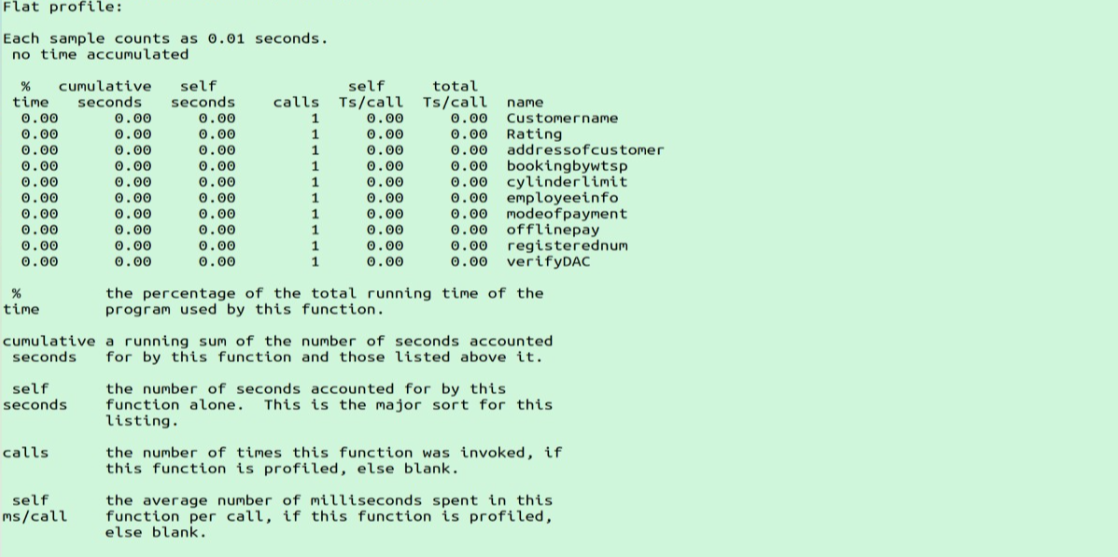
\includegraphics[width=\linewidth]{profiling 1-modified.png}
    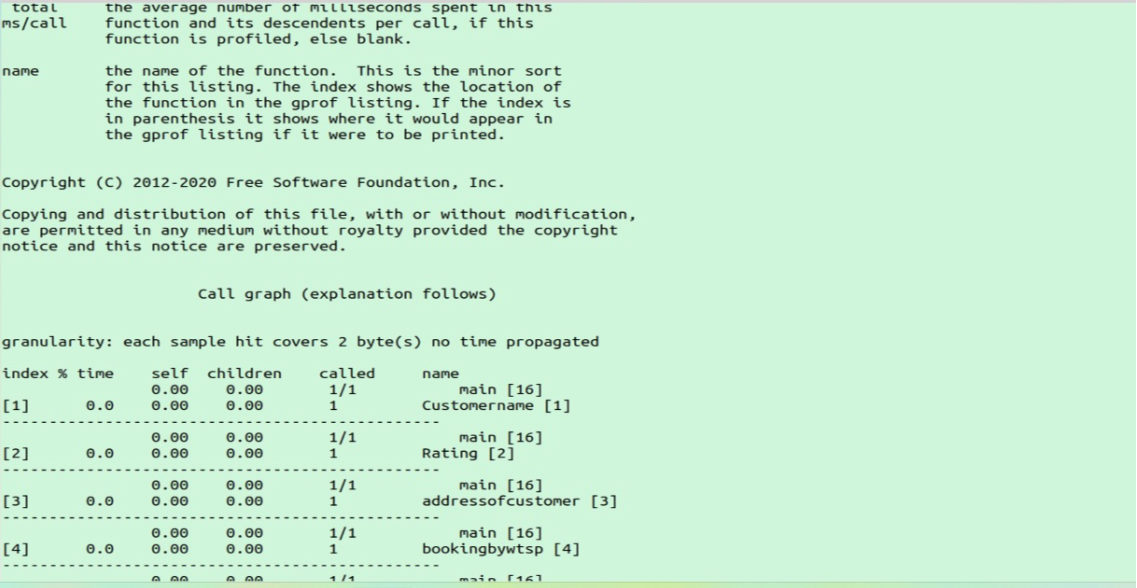
\includegraphics[width=\linewidth]{profiling 2-modified.png}
    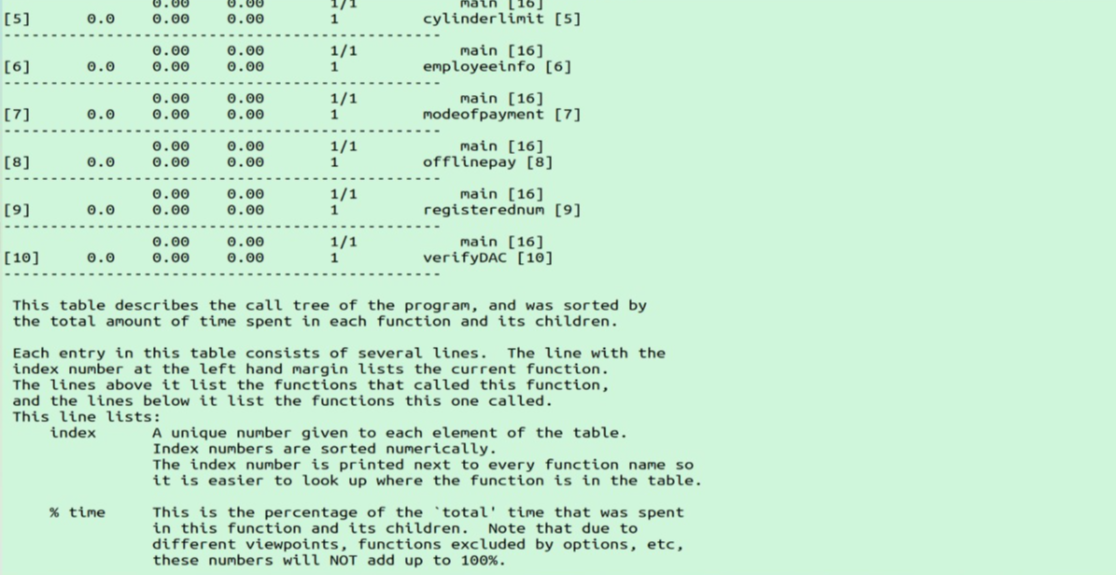
\includegraphics[width=\linewidth]{profiling 3-modified.png}
    \includegraphics[width=\linewidth]{profiling -modified.png}
    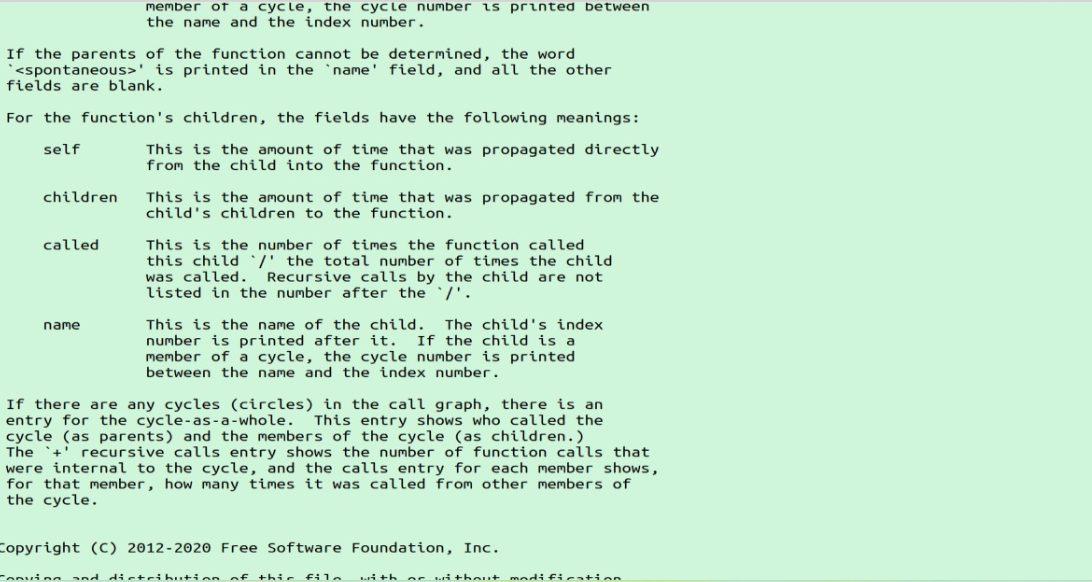
\includegraphics[width=\linewidth]{profiling 5-modified.png}
    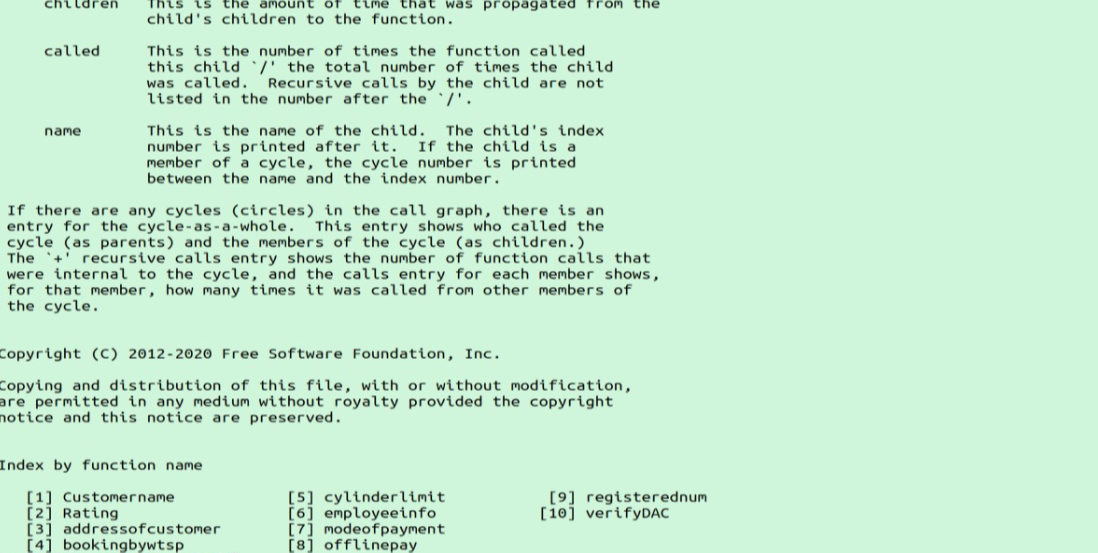
\includegraphics[width=\linewidth]{profiling 6-modified.png}
    \label{fig:my_label}
\end{figure}
\\
\\
\section{Debuggingg:}
\begin{figure}
    \centering
    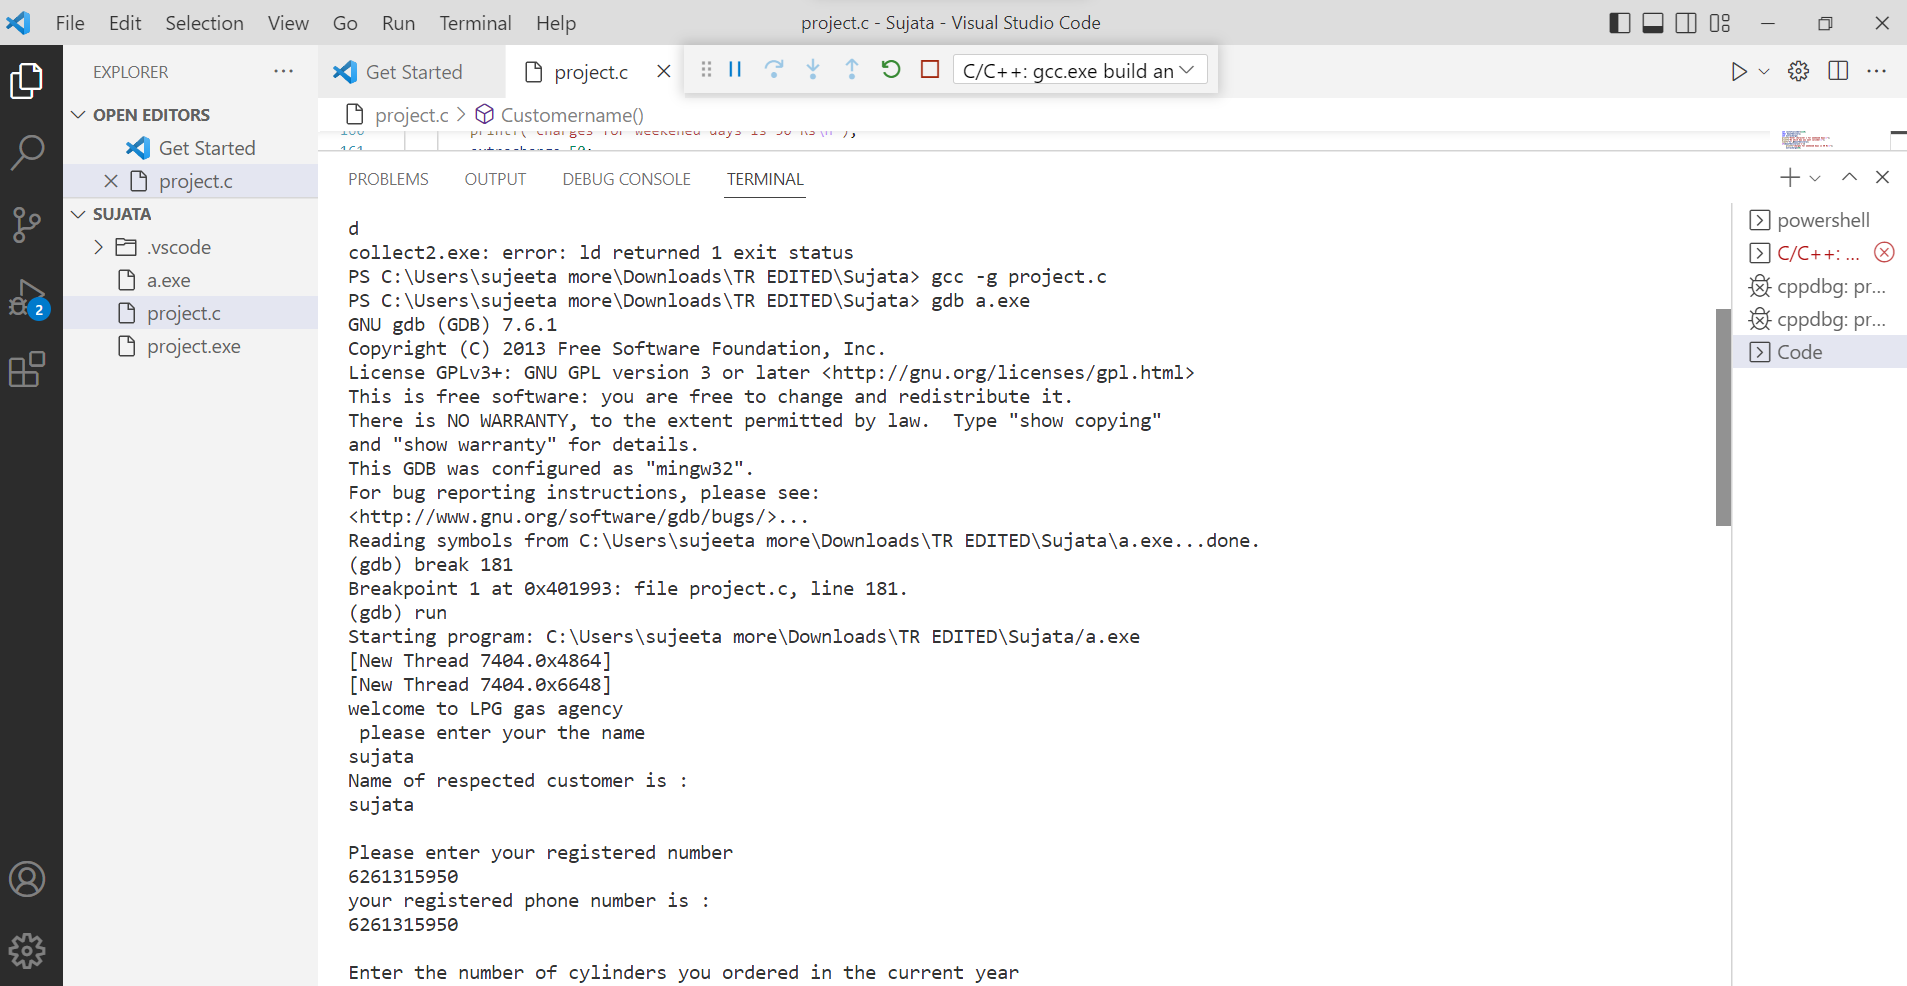
\includegraphics[width=\linewidth]{debug1.png}
    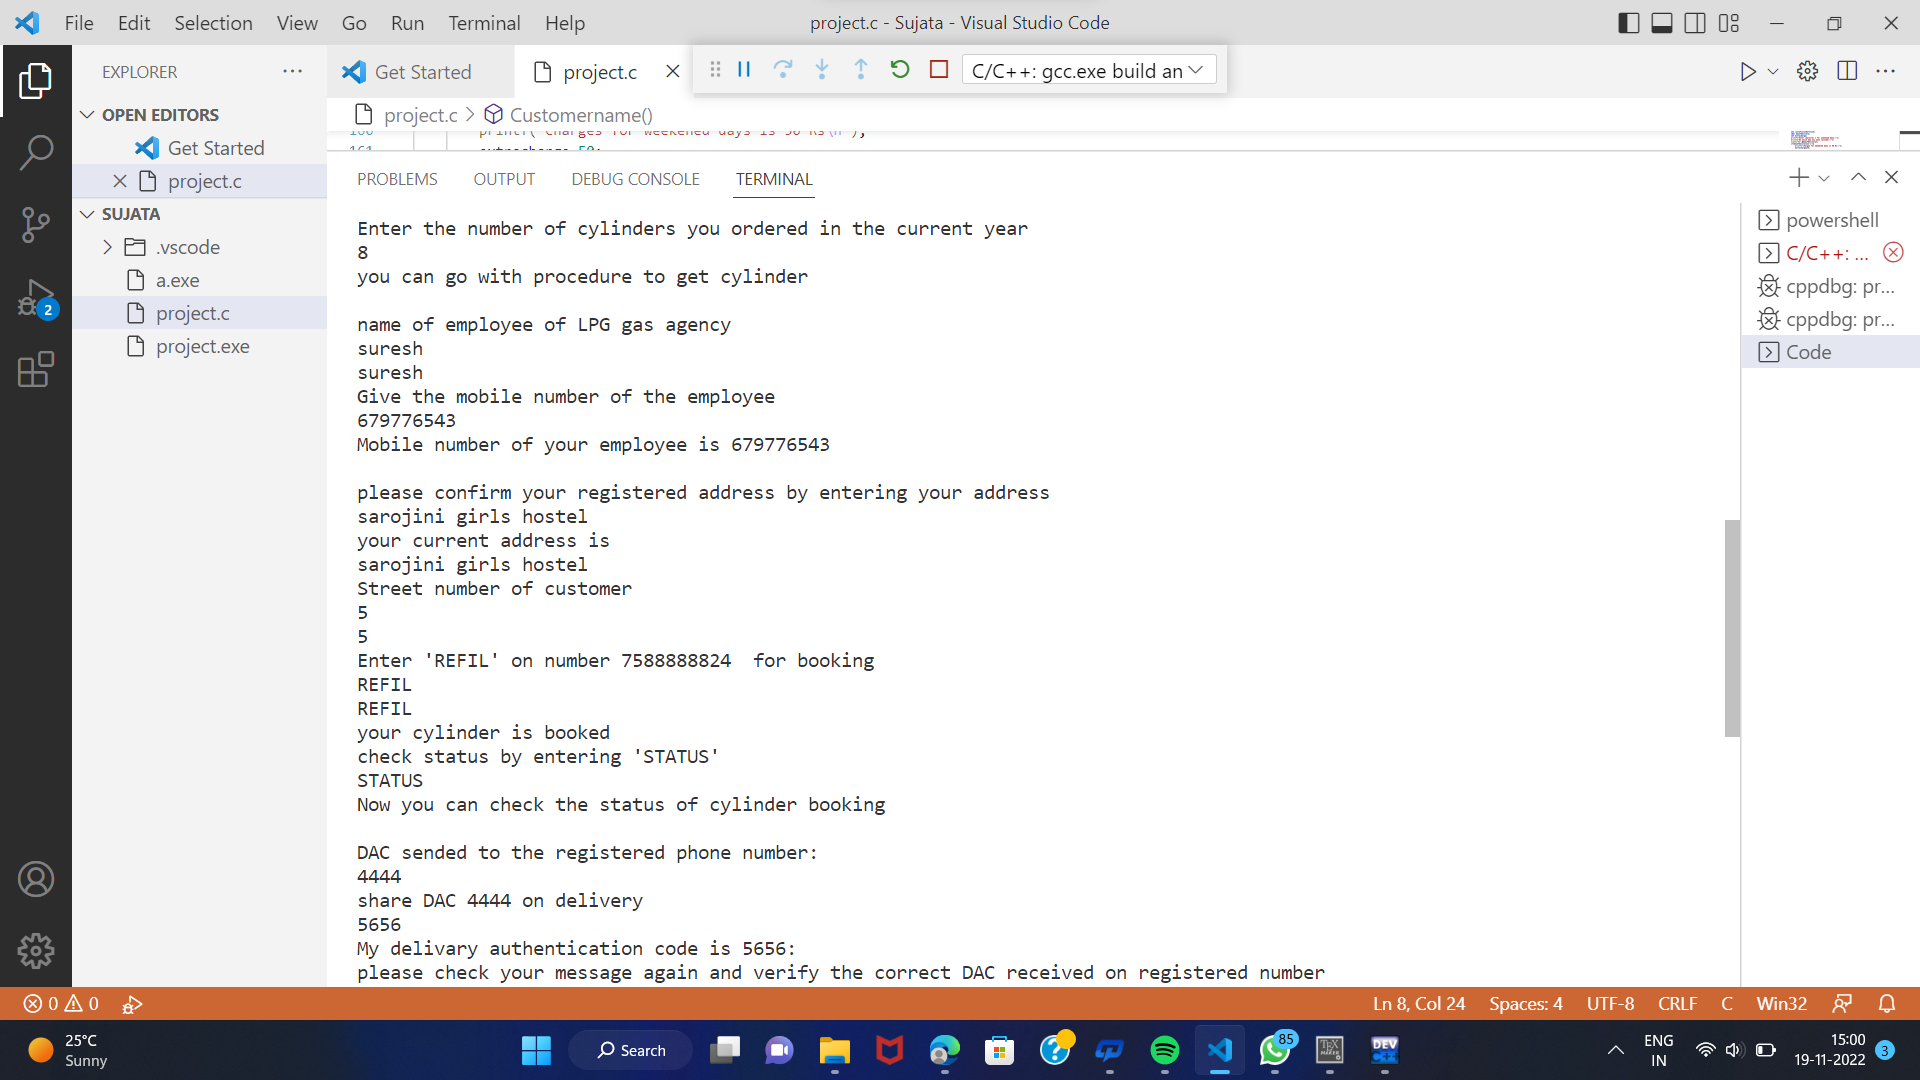
\includegraphics[width=\linewidth]{debug2.png}
    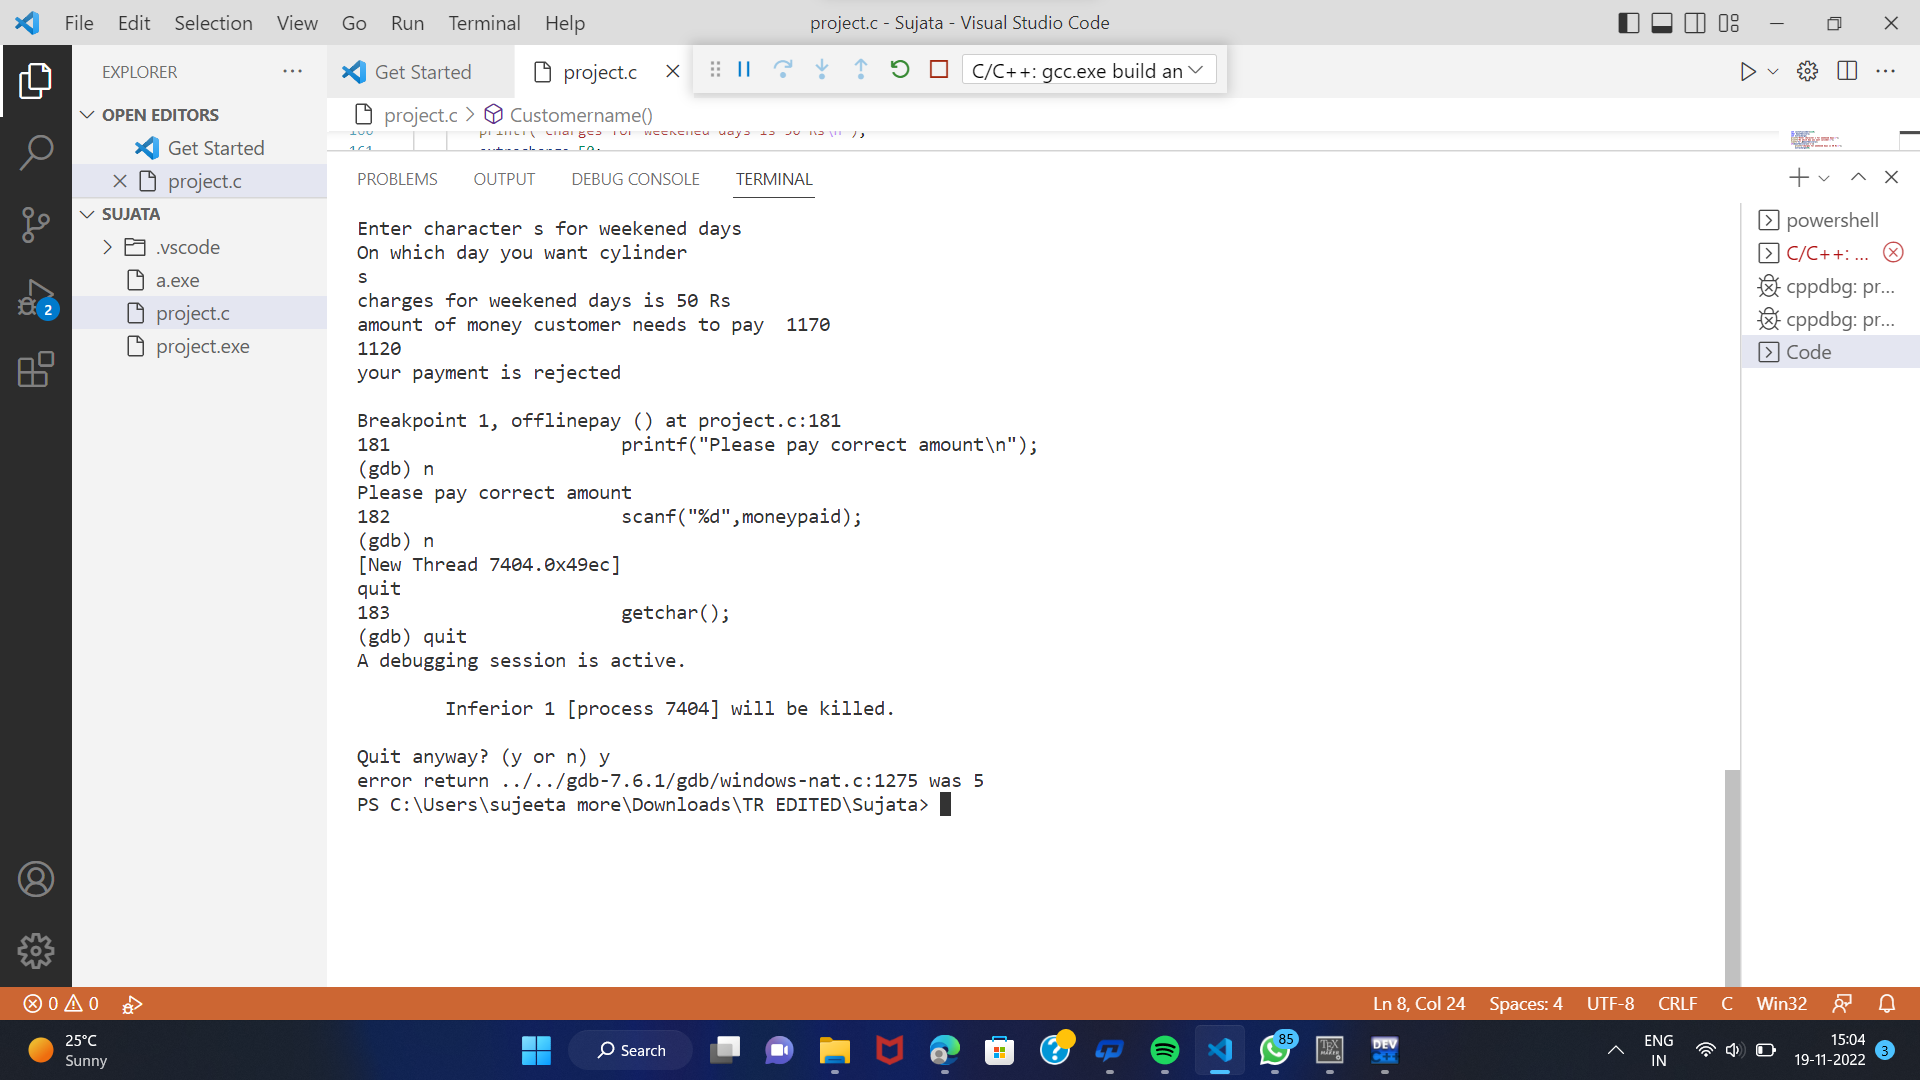
\includegraphics[width=\linewidth]{debug4.png}
    \label{fig:my_label}
\end{figure}
 \end{document}   